\documentclass[12pt,a4paper]{report}

%------Packages-----%
\usepackage{amsmath,amsfonts,amssymb,enumerate}
\usepackage[top=1in,bottom=1in,right=1in,left=1.5in]{geometry}
\usepackage{graphicx,titlesec}
\usepackage{hyperref,float}
\usepackage[]{url}
\usepackage{datetime,hanging}

%------Infos-----%
\author{FOE.41.008.014.21}
\title{Computer Lab II Report}
\newcommand{\lecturer}{Dr. AKYENE TETTEH}
\newcommand{\school}{
	\centering
	\textbf{\large UNIVERSITY OF MINES AND TECHNOLOGY \\TARKWA
	\vspace{1cm}	\\FACULTY OF COMPUTING AND MATHEMATICAL SCIENCES
	DEPARTMENT OF COMPUTER SCIENCE AND ENGINEERING
	}
}

\newcommand{\rpaim}{
	\centering

 \textbf{\large LITERATURE REVIEW OF TEN ARTICLES \\ REVIEW TOPIC\\REVOLUTIONIZING NETWORKS WITH SOFTWARE DEFINED NETWORKING \\BY \\FOE.41.008.014.21\\COURSE : RESEARCH METHODS AND ETHICS \\CE 352\\ LECTURER : \lecturer \\ \vspace{1.5cm} \today }}


%------Body-----%

\begin{document}
	\pagenumbering{roman}
	% School Info
	\begin{titlepage}
		\school
		\vspace{2cm}
		\begin{center}
			
\includegraphics[width=0.4\textwidth]{/home/kali/Documents/latex_files/School/umaru_report/umat_logo.jpg} % Adjust width as needed
		\end{center}
		\vspace{1cm}
		\rpaim

		\vfill

	%	\maketitle
	\end{titlepage}
	% Chapters
	\pagenumbering{arabic}
	\chapter*{\centering Task 1}
\addcontentsline{toc}{chapter}{Task 1}
	%\chapter*{\centering Task 2}
\addcontentsline{toc}{chapter}{Task 2}
\section*{ANTIVIRUS SOFTWARE INSTALLATION}
\begin{enumerate}
	\item
	Open your web browser and go to the official website of Avira antivirus software to download \url{https://www.avira.com}
	\begin{figure}[H]
		\centering
			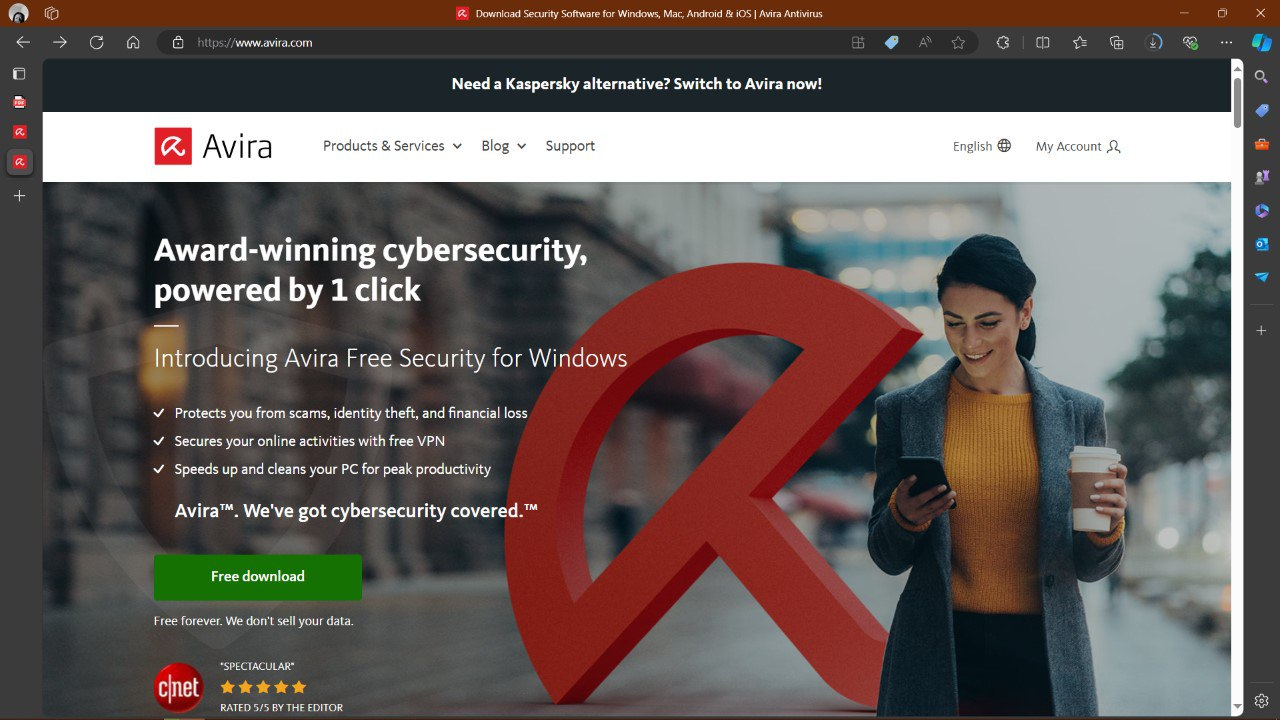
\includegraphics[scale=0.5,height=5cm]{"/home/kali/Documents/latex_files/cyber_rp/graphics/homepage.jpg"} \\
		\caption{Avira Homepage}
	\end{figure}
	\item
	Before installing Avira Antivirus ensure your operating system  is up to date by checking for updates via the “Settings” menu.Uninstalled  previous antivirus software to prevent any conflicts during installation.
	\begin{figure}
		\centering
		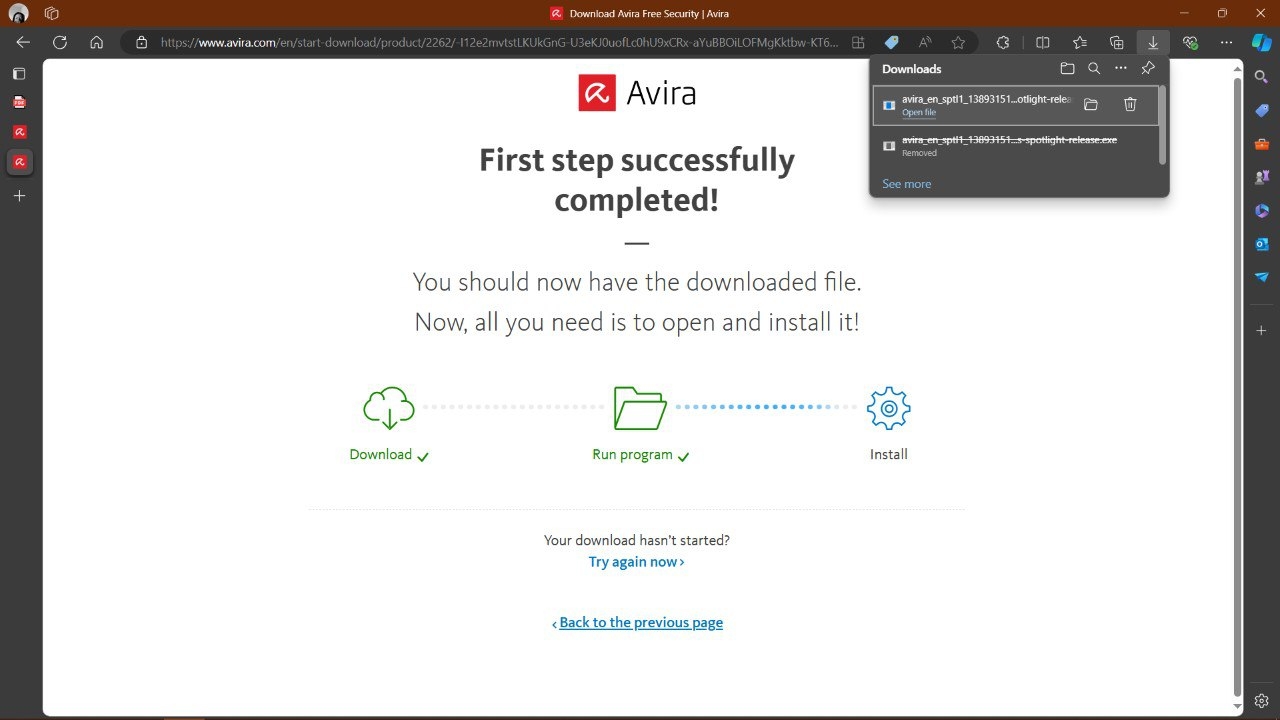
\includegraphics[scale=0.5,height=5cm]{"/home/kali/Documents/latex_files/cyber_rp/graphics/downprg.jpg"} \\

	\end{figure}
	\item
	Download and run the (avastfreeantivirussetuponline.exe)  installer using the download link provided.
	\item
	Launch and accept the End User License Agreement (EULA)  after reading through it.Choose the “Default Installation” option to keep things simple and let Avira install to the default location on your C: drive.The installation process will take a few minutes as Avira Antivirus copies files and configured settings.\\
		\begin{figure}[H]
		\centering
		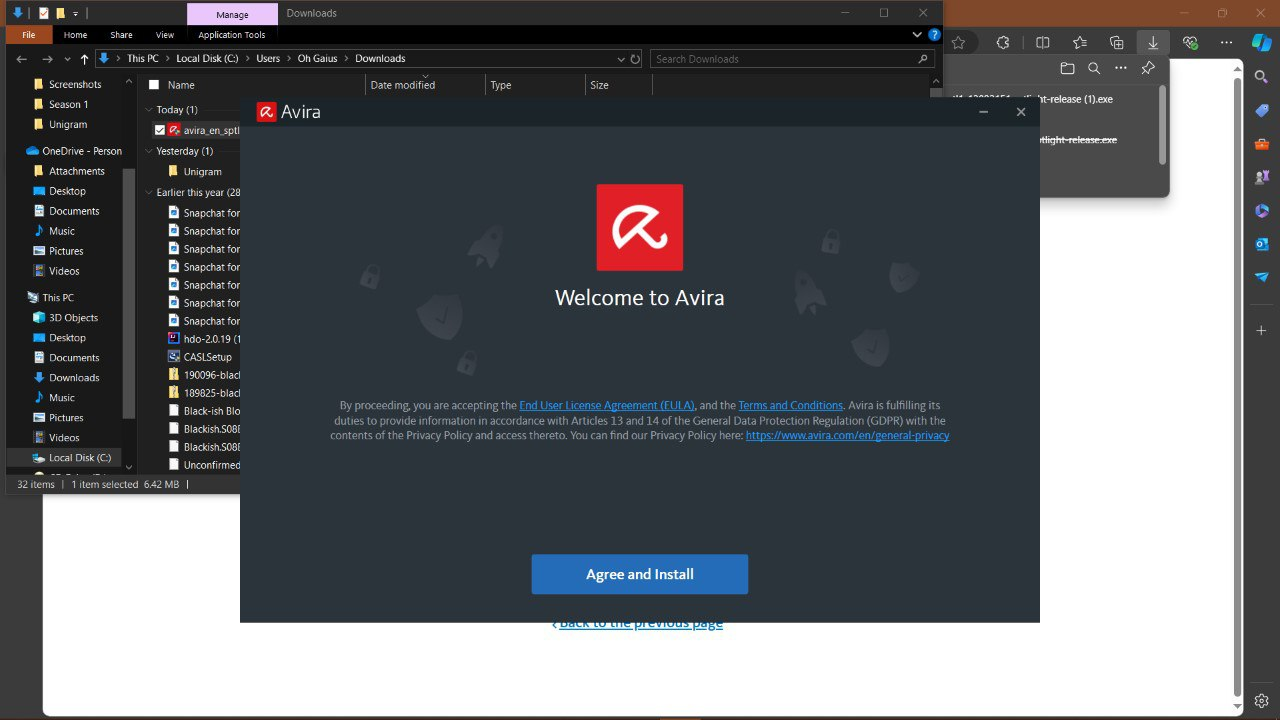
\includegraphics[scale=0.5,height=5cm]{"/home/kali/Documents/latex_files/cyber_rp/graphics/inst.jpg"} \\
		\caption{Avira Installation}
	\end{figure}
	\item
	Avira Antivirus automatically checks for updates whiles installing to ensure it has the latest virus definitions in the application.The update process is quick and takes only a couple of minutes to complete.
	\begin{figure}[H]
		\centering
		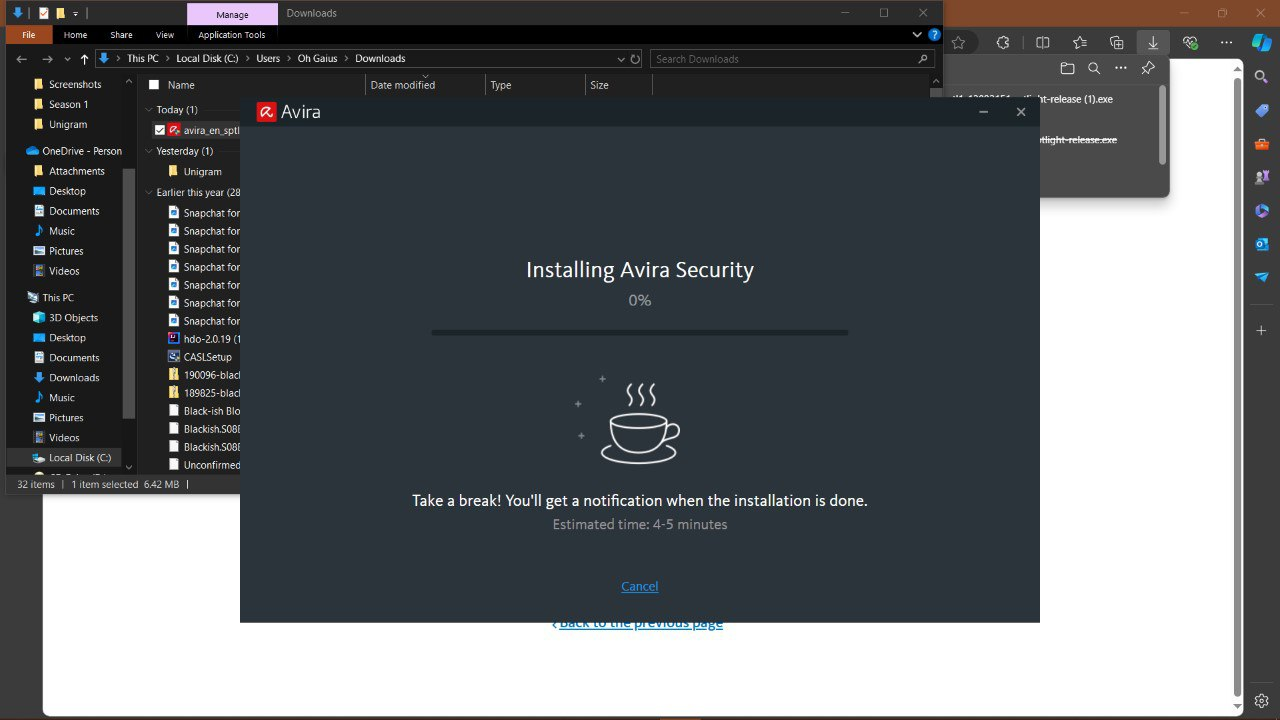
\includegraphics[scale=0.5,height=5cm]{"/home/kali/Documents/latex_files/cyber_rp/graphics/updatee.jpg"} \\
		\caption{Running Avira Update}
	\end{figure}
	\item
	Run Avira scan to check your pc against malware.
	\begin{figure}[H]
		\centering
		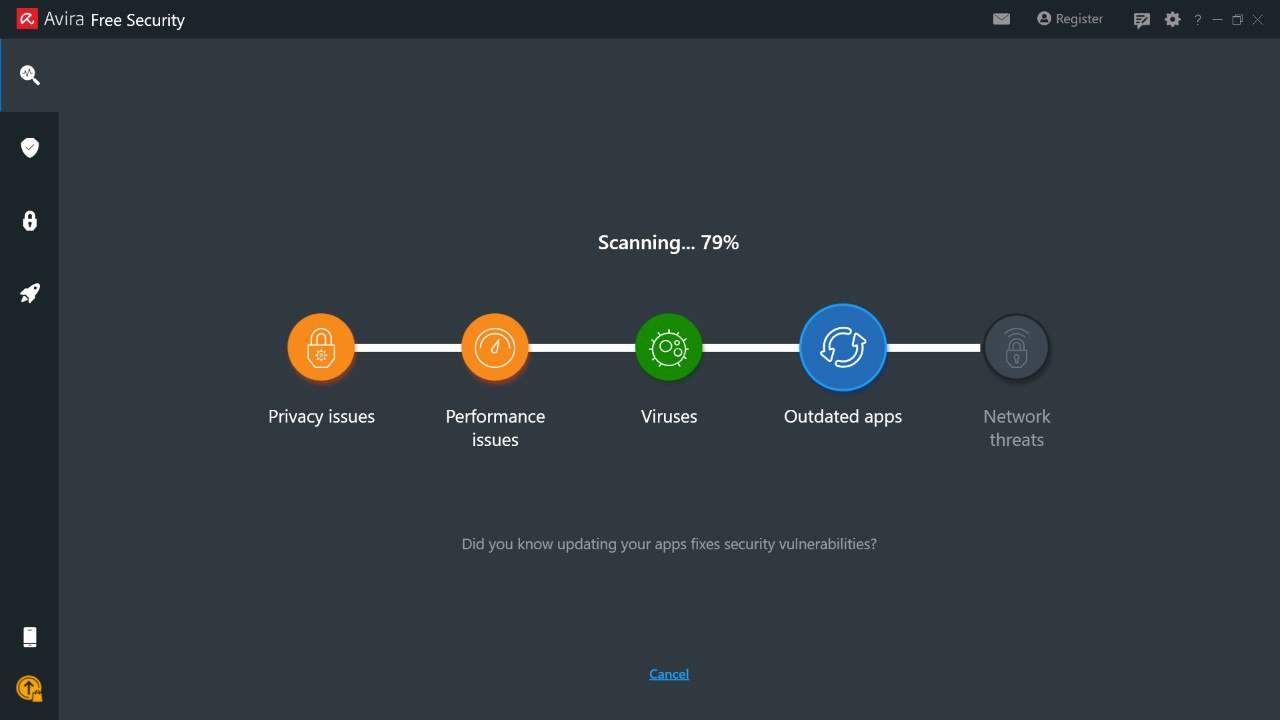
\includegraphics[scale=0.5,height=5cm]{"/home/kali/Documents/latex_files/cyber_rp/graphics/scann.jpg"} \\
		\caption{Scanning for malware}
	\end{figure}

\end{enumerate}

	% References
	\chapter{References}
References

	%------Conclusion-----%

\end{document}
